\documentclass[english,14pt]{beamer}
\usetheme{EastLansing}
\usecolortheme{spruce}

\usepackage{xcolor}
\usepackage{listings}
\usepackage{courier}
\usepackage{graphicx}
\usepackage{amsmath}
\usepackage{algorithm2e}
\usepackage{multicol}
\usepackage{hyperref}
\usepackage{textcomp}

% http://mirrors.ibiblio.org/CTAN/macros/latex/contrib/datetime2/datetime2.pdf
\usepackage{babel}
\usepackage[useregional]{datetime2}

% https://tex.stackexchange.com/questions/42619/x-mark-to-match-checkmark
\usepackage{pifont}% http://ctan.org/pkg/pifont

%% https://stackoverflow.com/questions/1435837/how-to-remove-footers-of-latex-beamer-templates
%%gets rid of bottom navigation bars
%\setbeamertemplate{footline}[page number]
%
%gets rid of navigation symbols
\setbeamertemplate{navigation symbols}{}


\usefonttheme[onlymath]{serif}

\definecolor{mGreen}{rgb}{0,0.6,0}
\definecolor{mGray}{rgb}{0.5,0.5,0.5}
\definecolor{mPurple}{rgb}{0.8,0,0.82}
\definecolor{backgroundColour}{rgb}{0.95,0.95,0.92}
\definecolor{lightBlue}{rgb}{0.1, 0.1, 0.8}
\definecolor{darkGreen}{rgb}{0, 0.39, 0}

\newcommand\red[1]{{\color{red} #1}}
\newcommand\green[1]{{\color{green} #1}}
\newcommand\blue[1]{{\color{blue} #1}}
\newcommand\darkGreen[1]{{\color{darkGreen} #1}}

\newcommand{\cmark}{\ding{51}}%
\newcommand{\xmark}{\ding{55}}%

\lstdefinestyle{CStyle}{
    backgroundcolor=\color{backgroundColour},   
    commentstyle=\color{mGreen},
    keywordstyle=\color{magenta},
    numberstyle=\tiny\color{mGray},
    stringstyle=\color{mPurple},
    basicstyle=\footnotesize,
    breakatwhitespace=false,         
    breaklines=true,                 
    captionpos=b,                    
    keepspaces=true,                 
    numbers=left,                    
    numbersep=5pt,                  
    showspaces=false,                
    showstringspaces=false,
    showtabs=false,                  
    tabsize=2,
    language=Python
}

\lstdefinestyle{MStyle}{
    backgroundcolor=\color{backgroundColour},   
    commentstyle=\color{mGreen},
    keywordstyle=\color{magenta},
    numberstyle=\tiny\color{mGray},
    stringstyle=\color{mPurple},
    basicstyle=\footnotesize,
    breakatwhitespace=false,         
    breaklines=true,                 
    captionpos=b,                    
    keepspaces=true,                 
    numbers=left,                    
    numbersep=5pt,                  
    showspaces=false,                
    showstringspaces=false,
    showtabs=false,                  
    tabsize=2,
    language=MATLAB
}

\lstdefinestyle{pseudo}{
        basicstyle=\ttfamily\footnotesize,
        keywordstyle=\color{lightBlue},
        morekeywords={BEGIN,END,IF,ELSE,ENDIF,ELSEIF,PRINT,WHILE,RETURN,ENDWHILE,DO,FOR,TO,IN,ENDFOR,BREAK,INPUT,CONDITIONS},
        morecomment=[l]{//},
        commentstyle=\color{mGreen}
}

\lstset{basicstyle=\footnotesize\ttfamily,breaklines=true}
\lstset{framextopmargin=50pt,tabsize=2}

\title{ENGG1003 - Thursday Week 12}
\subtitle{Final exam preparation}
\author{Steve Weller}
\institute{University of Newcastle}
%\date{\today}
\date{27 May 2021}

% following is a bit of a hack, but forces page numbers (technically: frame numbers) to run 1,2,3,... 
% with titlepage counting as frame 1

\addtocounter{framenumber}{1}
\titlepage

\begin{document}

\begin{flushleft}
{\scriptsize Last compiled:~\DTMnow}
\vspace*{-5mm}
\end{flushleft}
\framebreak

%==============================================================

\begin{frame}[fragile]

\frametitle{Lecture overview}
\begin{enumerate}
	\item Final exam organisational details
	\begin{itemize}
		\item when, how, how long, how much \ldots
		\item academic integrity
	\end{itemize}
	
	\item[]
	
	\item Overview of final exam questions
	\begin{itemize}
		\item Q1, Q2, Q3, Q4
%		\item Q2
%		\item Q3
%		\item Q4
	\end{itemize}

	\item[]
	
	\item Questions \& answers

	\item[]

\end{enumerate}

\end{frame}

%==============================================================

\begin{frame}[fragile]

\frametitle{1) Final exam organisational details}

\begin{itemize}
	\item \textbf{Date:} Tuesday 8 June
	\item \textbf{Time:} 2:00pm AEST
	\item \textbf{Location:} ONLINE exam, via Blackboard (BB)
	\item \textbf{Duration:} 130 minutes
	\begin{itemize}
		\item 2:00pm--4:10pm
	\end{itemize}
	\item final exam is \textbf{OPEN BOOK}
	\item[]
	\item counts for 35\% of overall course grade in ENGG1003
\end{itemize}

\begin{figure}[ht]
	\centering
	
\includegraphics[width=\textwidth]{figures/finalexamdatetime}
\end{figure}

\end{frame}

%==============================================================

\begin{frame}[fragile]

\frametitle{Final exam organisational details}

\begin{itemize}
	\item you will be asked to write Python code in the exam
	\begin{itemize}
		\item have your PyCharm setup prepared
	\end{itemize}
	\item[]
	\item the following resources ARE PERMITTED:
	\begin{itemize}
		\item lecture notes
		\item lab sheets
		\item notes, textbook, study guides
		\item pre-existing Python code, eg: developed for labs, quiz, assignments
		\item any pre-existing Internet resource
	\end{itemize}

	\item the following ARE NOT PERMITTED:
	\begin{itemize}
		\item assistance from friends, fellow students or any other person
		\item active participation in online forums
	\end{itemize}
	
\end{itemize}

\end{frame}

%==============================================================

\begin{frame}[fragile]

\frametitle{Academic integrity}

\begin{itemize}
	\item \href{https://policies.newcastle.edu.au/document/view-current.php?id=35&version=1}{Student Academic Integrity Policy}
	\item[]
	\item \href{https://policies.newcastle.edu.au/document/view-current.php?id=34}{Student Conduct Rule}
	\item[]
	\item cases of suspected collusion, plagiarism or other forms of academic misconduct will be reported to the School's \emph{Student Academic Conduct Officer (SACO)}
	\item[]
	\item Course Coordinators may need to perform an Oral Examination (Viva) with a student as a way of verifying the authorship of materials
\end{itemize}

\end{frame}

%==============================================================

\begin{frame}[fragile]

\frametitle{2) Overview of final exam questions}

\begin{itemize}
	\item exam consists of four (4) questions~$^\star$
	\begin{itemize}
		\item 10 marks per question
		\item marks indicated for parts (a),(b),(c) etc within a single question
	\end{itemize}
	\item[$\star$] \textbf{NOTE:} exact format of exam may differ to fit BB requirements
		\begin{itemize}
		\item will advise any changes to number of questions on BB/email/discord
		\item BUT will only be a \emph{re-organisation} of Q1--Q4
	\end{itemize}

	\item questions tend to get more difficult: Q1 ``easy'', Q2 slightly harder, Q3 harder again, Q4 hardest
	\item Q1 graded by BB, Q2--Q4 manually graded
\end{itemize}
\end{frame}

%==============================================================

\begin{frame}[fragile]

\frametitle{Question 1}

\begin{itemize}
	\item ten (10) multiple choice (1 mark each)
	\item[]
	\item given Python code, asked to:
	\begin{itemize}
		\item identify coding error (if any)
		\item what is the output when code runs? (if any)
		\item[]
		\item maybe other styles of multiple choice questions
	\end{itemize}
\end{itemize}

\end{frame}

%==============================================================

\begin{frame}[fragile]

\frametitle{}

{\small 
A student wrote the Python code below to calculate the sum total of all entries in array \texttt{x}. What happens when the code is run?}
\begin{figure}[ht]
	\centering
	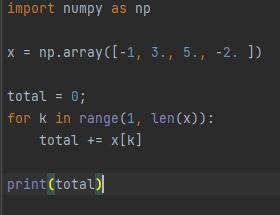
\includegraphics[width=.5\textwidth]{figures/sampleq1}
\end{figure}

\begin{itemize}
	\item[(a)] PyCharm \texttt{SyntaxError:~invalid syntax}
	\item[(b)] the code prints the total 5.0
	\item[(c)] the code prints the total 6.0
	\item[(d)] the code gets stuck in an infinite loop
\end{itemize}

\end{frame}

%==============================================================

\begin{frame}[fragile]

\frametitle{Question 2}

General scope of Q2 as follows \ldots

\vspace*{5mm}

Write Python code to:

\begin{itemize}
	\item evaluate an expression $f(x)$ at a single value of $x$
	\item evaluate an expression $f(x)$ at a range of values $x$ using \emph{loops}
	\item evaluate an expression $f(x)$ at a range of values $x$ using a \emph{vectorised solution}
	\item generate a plot
	\item put $x$-labels, $y$-labels, title, grid etc on plot
\end{itemize}

\end{frame}

%==============================================================

\begin{frame}[fragile]

\frametitle{Question 2}

Write a Python script to plot the following function:
\[
f(t) = e^{-at}\left( \sin(5t) + \cos(10t)\right)
\]
using $200$ linearly spaced time points over the range $0 \leq t \leq 5$. Your script should use the value $a = 2$. Display todays date in the title of the plot. Use of any Python library is permitted.

\begin{itemize}
\item[(a)] Upload your Python code to the submission box below
\item[(b)] Upload the plot image to the file upload box below
\end{itemize}

\end{frame}

%==============================================================

\begin{frame}[fragile]

\frametitle{Question 3}

\begin{itemize}
	\item xxx
\end{itemize}

\end{frame}

%==============================================================

\begin{frame}[fragile]

\frametitle{Question 4}

\begin{itemize}
	\item xxx
\end{itemize}

\end{frame}

%==============================================================

\begin{frame}[fragile]

\frametitle{3) Questions \& answers}

\begin{itemize}
	\item xxx
\end{itemize}

\end{frame}

\end{document}